\documentclass[10pt,a4paper]{article}
\usepackage[utf8]{inputenc}
\usepackage[english]{babel}
\usepackage{graphicx}
\usepackage{lmodern}
\usepackage{kpfonts}
\usepackage{subcaption}
\usepackage{dsfont}
\usepackage{wrapfig}
\usepackage[left=2cm,right=2cm,top=2cm,bottom=2cm]{geometry}
\author{Megi Dervishi}
\title{Machine Learning Homework 2}
\begin{document}
\maketitle
\section*{Exercise 1}
\begin{enumerate}
\item[\textbf{(a)}]  Overfitting is especially a big problem when the training data size is low and the number of features to learn is very large compared to the data. By regularizing you avoid the risk of overfitting and hence have a better accuracy in the test data. So by choosing a good $\lambda$ regularization significantly reduces the variance of the regression model without a huge increase in the bias of it. In this case the number of features are $784$ while the training data has 900 images and the testing data has $250$ images.
\item[\textbf{(b)}] I used the proximial gradient descent algorithm also known as ISTA for finding the $\theta_{\lambda}$ for the $\ell_1$ norm and applied directly Gradient Descent for the $\ell_2$ norm. For both graphs the increase of $\lambda$ results in the increase of error. This is normal because if $\lambda$ becomes too high then the bias of the model increases which results in lower accuracy. Also note that for the $\ell_1$ norm the error increases much faster than for the $\ell_2$ norm.

\begin{figure}[h!]
\centering
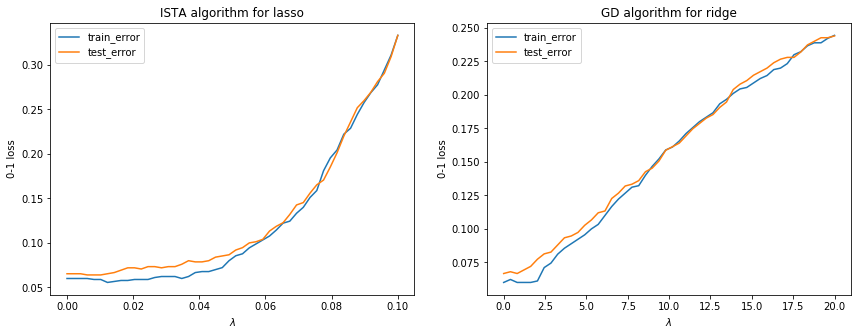
\includegraphics[width = 0.7\textwidth]{graph1.png}
\caption{Error for the ISTA algorithm with $||\cdot||1$ penalty (left) and GD algorithm with $||\cdot||_2^2$ penalty (right).}
\end{figure}
 
\item[\textbf{(c)}] In order to  best tune $\lambda$ I performed K - fold cross validation which resulted with the following best lambdas:
$$ \lambda_{lasso} = 0.011 \quad \quad \lambda_{lasso} = 0.588$$

\item[\textbf{(d)}]
\begin{figure}[h!]
\centering
\begin{subfigure}[b]{0.5\textwidth}
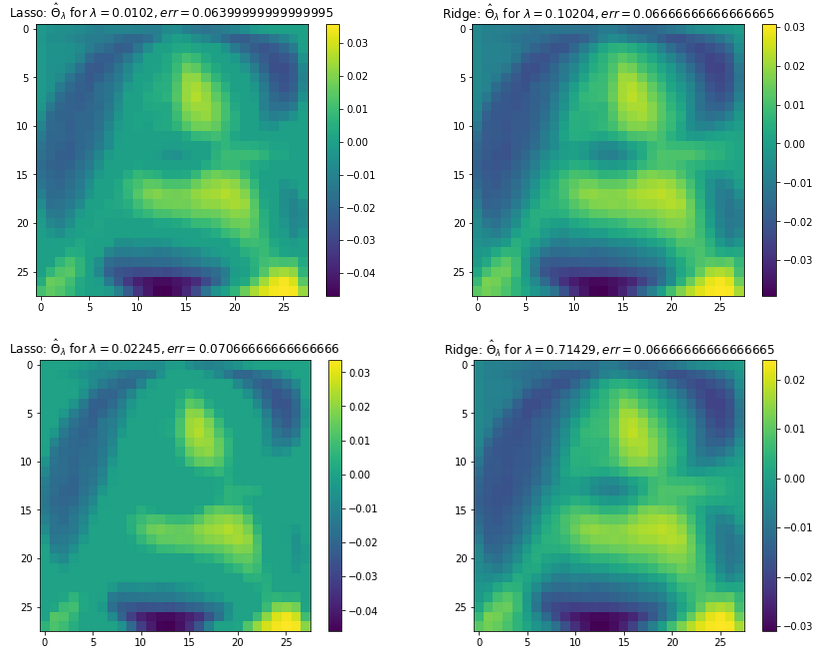
\includegraphics[width = 0.7\textwidth]{estimators.png}
\caption{.}
\end{subfigure}
\begin{subfigure}[b]{0.5\textwidth}
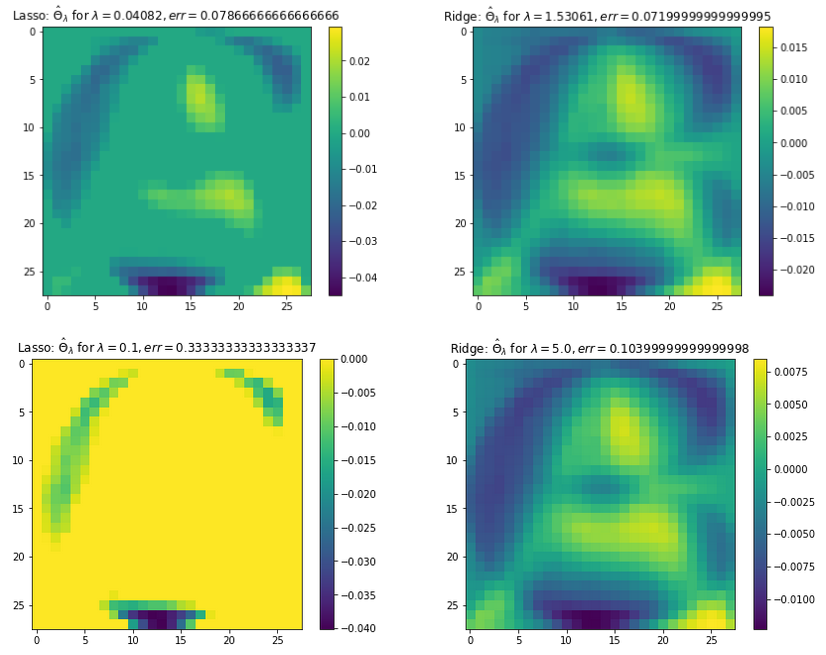
\includegraphics[width = 0.7\textwidth]{estimators2.png}
\caption{.}
\end{subfigure}
\end{figure}

\end{enumerate}

\section*{Exercise 2}
\begin{enumerate}
\item[\textbf{(a)}]
By Baysian Law we get the result (1). By law of total probability we find  $\mathbb{P}[X=x]$and substitute it back into (1) which gives the final result (2): 
\begin{align}
\mathbb{P}[Y = 1| X]] &= \frac{\mathbb{P}[X=x | Y =1] \, \mathbb{P}[Y =1]}{\mathbb{P}[X = x]} = \frac{\mathcal{N}(\mu_1, \Sigma)(x) \cdot \pi}{\mathbb{P}[X = x]}
\end{align}
\begin{align*}
\mathbb{P}[X = x] &=  \mathbb{P}[X = x | Y = 1] \, \mathbb{P}[y = 1] +  \mathbb{P}[X = x | Y = -1] \, \mathbb{P}[y = -1] \\
&= \mathcal{N}(\mu_1, \Sigma)(x)\pi + \mathcal{N}(\mu_{-1}, \Sigma)(x)(1-\pi)
\end{align*}
\begin{align}
\frac{\mathcal{N}(\mu_1, \Sigma)(x) \cdot \pi}{\mathbb{P}[X = x]}  = \frac{1}{1+ \frac{\mathcal{N}(\mu_{-1}, \Sigma)(x) \cdot (1- \pi)}{\mathcal{N}(\mu_1, \Sigma)(x) \cdot \pi}}
\end{align}
By substituting the normal density function and simplifying we have (3). Now we want to transform (3) into something of the form $\exp (- \beta_0 - \langle \beta, x\rangle) = \exp ( - \beta_0 - tr( \beta^T x ))$:
\begin{align}
\frac{\mathcal{N}(\mu_{-1}, \Sigma)(x) \cdot (1- \pi)}{\mathcal{N}(\mu_1, \Sigma)(x) \cdot \pi} &=\exp (-\frac{1}{2}(x-\mu_{-1})^T \Sigma ^{-1} (x- \mu_{-1}) +\frac{1}{2}(x-\mu_{1})^T \Sigma ^{-1} (x- \mu_{1}) + \log(\frac{1-\pi}{\pi}))
\end{align}
\begin{align*}
&=  \exp(\frac{1}{2}(\mu_{-1}^T\Sigma^{-1}x + x^T \Sigma ^{-1} \mu_{-1}) + \frac{1}{2}(-\mu_{1}^T\Sigma^{-1}x - x^T \Sigma ^{-1} \mu_{1}) + 
\frac{1}{2}(\mu_1^T\Sigma^{-1}\mu_{1} -\mu_{-1}^T\Sigma^{-1}\mu_{-1} ) + \log (\frac{1-\pi}{\pi}))\\
&= \exp(\frac{1}{2}(\mu_{-1}^T\Sigma^{-1}x + \mu_{-1}^T \Sigma ^{-1} x) + \frac{1}{2}(-\mu_{1}^T\Sigma^{-1}x - \mu_{1}^T \Sigma ^{-1} x) - ( \underbrace{
\frac{1}{2}(\mu_{-1}^T\Sigma^{-1}\mu_{-1} +\mu_{1}^T\Sigma^{-1}\mu_{1} ) - \log (\frac{1-\pi}{\pi})}_{\beta_0})) \\
&= \exp((\mu{-1}^T\Sigma^{-1} + \mu_{1}^T\Sigma^{-1} )x - \beta_0)\\
&=  \exp(-(\mu_{1}^T\Sigma^{-1} - \mu_{-1}^T\Sigma^{-1} )x - \beta_0)\\
&= \exp(- \beta^T x - \beta_0)
\end{align*}
Since $- \beta^T x$ is a value then it is equal to $tr(- \beta^T x)$. We finally conclude that indeed: $$\mathbb{P}[Y = 1 | X] =\frac{1}{1+ \exp \,(-\beta_0 - \langle \beta, X \rangle )} $$

\item[\textbf{(b)}] We have that:
\begin{align}
\mathcal{L}(\beta_0 , \beta) = \prod ^n _{j=1} \mathbb{P}[Y = y_j | X = x_j] = \prod ^n_{j=1} \frac{1}{1+\exp (-y_j \beta_0 - y_j \langle \beta, x_j \rangle)}
\end{align}
The reason behind the second equality is because we notice that $\mathbb{P}[Y = -1 | X] =\frac{1}{1+ \exp \,(\beta_0 + \langle \beta, X \rangle )} $ and by (a) we can generalize $\mathbb{P}[Y = j | X = x_j]$ to the above expression. We have to maximize (4) in other words find ${\text{arg}}\max\limits_{\beta \in \mathbb{R}^d}(\mathcal{L}(\beta_0, \beta))$. Since $log$ is an increasing function we can take the log of the likelihood. Hence:
\begin{align*}
{\text{arg}}\max\limits_{\beta \in \mathbb{R}^d}\,\log(\mathcal{L}(\beta_0, \beta)) &= {\text{arg}}\max\limits_{\beta \in \mathbb{R}^d} \, \sum^{n}_{j=1} \log(\frac{1}{1+ \exp \,(\beta_0 + \langle \beta, X \rangle })\\
& = {\text{arg}}\max\limits_{\beta \in \mathbb{R}^d} \, - \sum^{n}_{j=1} \log(1+ \exp \,(\beta_0 + \langle \beta, X \rangle )\\
&= {\text{arg}}\min\limits_{\beta \in \mathbb{R}^d} \frac{1}{n}\sum^{n}_{j=1} \log(1+ \exp \,(\beta_0 + \langle \beta, X \rangle )\
\end{align*} 
If we let $\beta_0 = 0$ then this corresponds to the solution of logistic regression with $\lambda = 0$. Note(since $\frac{1}{n}$ is a constant adding it to ${\text{arg}}\min$ does not change). 

\item[\textbf{(c)}]
For the algorithm that I implemented I based myself on the following: https://eigenfoo.xyz/lda/.


\item[\textbf{(d)}]  False positive means that you predict positive when the correct answer is false and False negative means that you predict negative when the correct answer is true. A classification error simply describes the ratio between the number of wrongly predicted values and the total number of values. The confusion matrix shows the ways in which your model was confused. In other words it gives more insights on which label was wrongly predicted i.e. when do you have false positive or false negative. By having these extra information you could pin-point better where the error comes from and perhaps improve it.
\end{enumerate}

\section*{Exercise 3}
\begin{enumerate}
\item[\textbf{(a)}] Since we are doing unsupervised learning I have reloaded the data into one and reshuffled it. The dataset is composed by 1650 of 28 by 28 pixels images which are normalized. Hence the input space is $\mathcal{X} \in [0,1]^{784}$ and $\mathcal{Y} \in \{0, 1, 2\}$ i.e. the image will have a label  $Y_i = 0$ if it shows "A", 1 if it shows "B" and 2 if it shows "C".  In figure a y


\item[\textbf{(b)}] You get an error of 20\% which may seem as if it is a lot. However when looking at the confusion matrix we observe that the model mostly confuses the "B" and "C" and is always good at separating them between "A".
\end{enumerate}



\end{document}